\documentclass[a4paper,11pt,exos]{nsi} % COMPILE WITH DRAFT
\usepackage{pifont}
\usepackage{fontawesome5}
\usepackage{hyperref}

\pagestyle{empty}

\begin{document}
\classe{\terminale Comp}
\titre{Paradoxe de l'inspection}
\maketitle

Julie est inspectrice dans un réseau de transport urbain. Elle contrôle régulièrement une ligne de bus, sur laquelle on annonce un temps de 10 min entre deux passages. Si elle arrive à un moment au hasard, son temps d'attente moyen devrait logiquement être de 5 min.\\
Pourtant, Julie a la sensation qu'elle attend en moyenne plus de 5 min.\\[.5em]
On étudie une situation dans laquelle six bus se présentent sur un intervalle de 60 min et le dernier bus arrive exactement à 60 min.

\subsection*{Partie A - Un bus toutes les 10 min}
Dans l'idéal, les bus arrivent toutes les 10 min exactement. On représente la situation par le schéma suivant :
\begin{center}
    \begin{tikzpicture}[xscale=0.2, yscale=1]
  % Axe principal
  \draw[thick,->] (0,0) -- (70,0); % flèche à droite
  % Graduations et labels
  \foreach \x in {0,10,...,60} {
    \draw[thick] (\x,0.2) -- (\x,-0.2);
    \node[below] at (\x, -0.2) {\x};
  }
  \foreach \x in {10,20,...,60} {
    \node[above] at (\x, 0.2) {\color{UGLiOrange}{\faBus}};
  }
\end{tikzpicture}
\end{center}


\begin{enumerate}
    \item Quelle est la probabilité que Julie arrive entre le premier et le deuxième bus ?
    \item Si Julie se présente entre le premier et le deuxième bus de façon aléatoire, quel est son temps d'attente moyen ?
    \item De même, pour chaque intervalle entre deux bus (et entre l'instant 0 et le premier bus), préciser la probabilité que Julie arrive pendant cet intervalle puis le temps d'attente moyen.
    \item En déduire la moyenne du temps d'attente sur la période de 60 min, dans cette situation.
\end{enumerate}

\subsection*{Partie B - La pire des situations}
On suppose que les six bus ont été bloqués sur le trajet et arrivent tous ensemble au bout de 60 min.\\
Julie se présente de façon aléatoire pendant cette période de 60 min. Calculer sont temps d'attente moyen.

\subsection*{Partie C - De nouveaux écarts}
On considère maintenant, à titre d'exemple, la situation où les bus arrivent à 8 min, 19 min, 22 min, 25 min, 36 min et 60 min. On représente la situation par le schéma suivant :
\begin{center}
    \begin{tikzpicture}[xscale=0.2, yscale=1]
  % Axe principal
  \draw[thick,->] (0,0) -- (70,0); % flèche à droite
  \foreach \x in {0,10,...,60} {
    \draw[thick] (\x,0.2) -- (\x,-0.2);
  }
  \node[below] at (0, -0.2) {0};
  \foreach \x in {8,19,22,25,36,60} {
    \node[above] at (\x, 0.2) {\color{UGLiOrange}{\faBus}};
    \draw[UGLiOrange,thick] (\x,0.2) -- (\x,-0.2);
    \node[below] at (\x, -0.2) {\color{UGLiOrange}{\x}};
  }
\end{tikzpicture}
\end{center}

\begin{enumerate}
    \item Pour chaque écart entre deux bus, calculer la probabilité que Julie arrive pendant cet intervalle et son temps d'attente moyen.
    \item En déduire la moyenne du temps d'attente sur la période de 60 min, dans cette situation.
\end{enumerate}

\subsection*{Partie D - Des écarts aléatoires}
On considère maintenant que les bus arrivent à des instants aléatoires :
\begin{enumerate}[label=\textbullet]
    \item le bus 1 arrive à un instant aléatoire entre 0 et 60 min,
    \item le bus 2 arrive à un instant aléatoire entre le bus 1 et 60 min,
    \item le bus 3 arrive à un instant aléatoire entre le bus 2 et 60 min,
    \item etc.
\end{enumerate}
Compléter le tableur suivant pour calculer le temps d'attente moyen de Julie. 
\begin{center}
    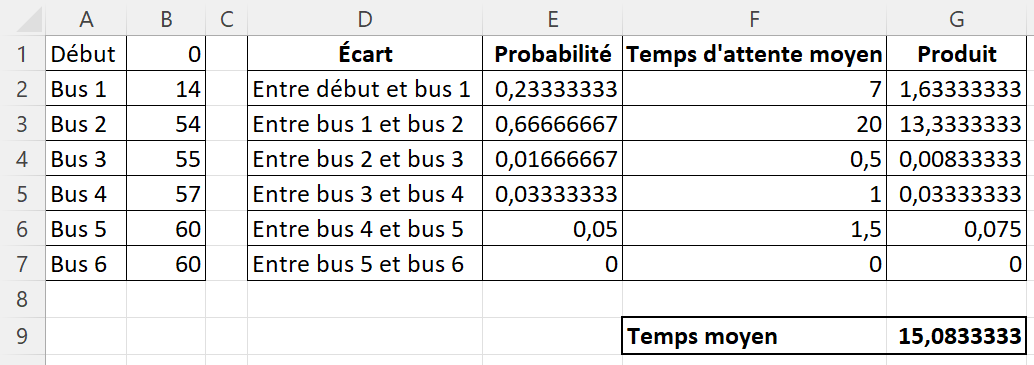
\includegraphics[width=12cm]{Paradoxe.png}
\end{center}
Observer les temps moyens obtenus. Que constate-t-on ?
\end{document}